\chapter{绪论}
\section{基本概念}
\subsection{技术(重点)}
是为了满足社会发展需要,运用科学的知识,在改造、控制、协调多种要素的实践活动中创造的劳动手段、工艺方法与技能体系的总称。

\subsection{经济(重点)}
(1)社会生产关系或国民经济的总称。例:工业经济、农业经济等;

(2)社会生产和再生产过程。例:生产、分配、交换、消费等;

(3)经济活动的合理性,即社会劳动的节约、节省或局部生产中的投入产出关系。例:经济效果、经济效益。

注意:《技术经济与工程管理》,此处经济指第3种含义。

\subsection{技术与经济的关系}
相互依赖、相互发展、相互制约。

技术和经济是人类社会物质生产时不可缺少的两个方面,任何一项技术的实施和采用都必须耗用一定的人、财、物,两者既有统一,又有矛盾,既互相联系,又互相制约,既考虑技术进步,先进性,又要考虑经济可行、合理性。

下面有一个简单的题。通过调查研究,设计以下备选方案:
\begin{longtable}{ccc}
\toprule
备选方案 & 学生离学校距离(公里) & 投资额(万元) \\
\midrule
\endfirsthead
\toprule
备选方案 & 学生离学校距离(公里) & 投资额(万元) \\
\midrule
\endhead
\midrule
\multicolumn{3}{r}{{续表}}\\
\endfoot
\bottomrule
\endlastfoot

1. & 1.0 & 6.0 \\
2. & 0.8 & 5.0 \\
3. & 1.2 & 4.4 \\
4. & 2.0 & 3.6 \\
5. & 1.5 & 4.4 \\
\end{longtable}


通过观察以上表格,你首先会排除哪几个方案呢?你最可能选择哪个方案?

这里用到了一种思想,叫做\textbf{帕累托最优}(Pareto Optimality),也称为帕累托效率(Pareto efficiency),是指资源分配的一种理想状态,假定固有的一群人和可分配的资源,从一种分配状态到另一种状态的变化中,在没有使任何人境况变坏的前提下,使得至少一个人变得更好,这就是帕累托改进或帕累托最优化。帕累托最优状态就是不可能再有更多的帕累托改进的余地。

上面一段话可能比较难以理解,我们把它简化一下。帕累托最优解就是,在给定的方案中,如果没有其他的方案在方方面面都比该方案好,那么该方案一定是一个帕累托最优解,即一个非劣解。反之,如果有其他的方案“在方方面面都比该方案好好”或“有些方面比该方案好,有些方面和该方案一样”,那么该方案就不是一个帕累托最优解,即是一个劣解。

在这个例子中,通过比较,可以得出方案1、5为劣解,方案2、3、4为非劣解。

最佳方案的选择(取决于决策者的愿望和倾向性):

(1)如认为就近入学是关键,且费用在4.5万元以下即可,则选方案3;

(2)如认为就近入学是关键,且扩建费用6.0万元以下即可,则选方案2;

(3)如认为扩建费用是关键,即越少越好,则选方案4;

(4)如认为就近入学和扩建费用二者综合考虑,则选方案3。

\subsection{技术经济分析过程}
\begin{figure}[H]
    \centering
    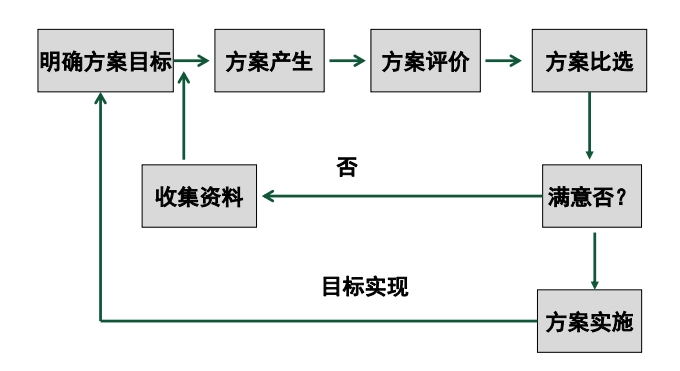
\includegraphics[width=0.8\textwidth]{image/微信截图_20241108214112.png}
    \caption{技术经济分析过程}
    \label{fig:3}
\end{figure}

\textbf{1. 确定目标功能:这是建立方案的基础。}

若我们预计缺30万kw电力,那么我们就要建立一个方案来满足30万kw电力的需要;

若某公司现有3亿元资金寻找投资方向,其目的只有一个:取得较好的回报率,那么我们就要提出一系列投资方案,最终的回报率要达到或超过预期回报率。

\textbf{2. 提出备选方案}

为达到一定目标,必须提出很多方案,如为了解决能源问题可以建火电厂、核电厂或水电站,而建核电站就有许多方案,如采用重水式的、轻水式的……

寻找备选方案,实际上是一项创新活动。人们要求决策者能针对某一特定的问题提出“最优”的解决方法,因而决策者必须创新。

\textbf{3. 方案评价}

方案要经过系统的评价,依据是政策法令与反映决策者意愿的指标体系。如产品要符合国家的产业政策、质量标准;

在符合基本条件后,最重要的是要有较好的经济效益和社会效益。

\textbf{4.选择最优方案}:树立系统观念和动态观念。


\subsection{项目(重点)}
国际项目管理协会(IPMA):项目是\textbf{受时间和成本约束的}、用以实现一系列既定的可交付物(达到项目\textbf{目标}的范围)、同时满足质量标准和需求的\textbf{一次性活动}。

\subsection{项目可行性研究}
项目可行性研究是对项目在投资决策前进行技术经济论证的一门综合性技术。它的任务是\textbf{以市场为前提,以技术为手段,以经济效益为最终目标},对拟建的项目从必要性、可能性、有效性和合理性等方面进行全面、系统地论证,做出项目可行或不可行的评价。

\subsection{财务评价(重点)}
根据国家现行的财税制度和价格体系,在财务效益与费用的估算以及编制财务辅助报表的基础上,编制财务报表,计算财务分析指标,考察和分析项目的\textbf{盈利能力、偿债能力和财务生存能力},判断项目的财务可行性,明确项目对财务主体的价值以及对投资者的贡献,为投资决策、融资决策以及银行贷款等提供依据。

考点1:请你说明什么是盈利能力评价指标,什么是偿债能力评价指标,什么是财务生存能力评价指标。(考察概率小)

答:盈利能力评价指标是用于衡量企业获取利润的能力的指标,反映了企业在一定时期内的收益水平。偿债能力评价指标是指企业偿还各种债务的能力的指标,分为短期偿债能力指标和长期偿债能力指标。财务生存能力评价指标主要是评估企业是否有足够的资金维持正常的生产经营活动,确保企业在一定时期内的资金收支平衡。

考点2:项目财务评价的概念、财务评价重点考查的三种能力是什么?

答:\textbf{盈利能力、偿债能力、财务生存能力}。

考点3:请你说明项目财务评价的作用是什么。

答:考察项目的财务盈利能力;制定项目资金规划的依据;银行发放贷款的重要依据;为协调国家利益和企业利益提供依据。